\documentclass{article}
\usepackage{graphicx}
\begin{document}
\title{Some Investigations in standardisation with $t_2$}
\maketitle
In this report, I summarise a short test I carried out to see the distributions in $\sigma_{res}$ for two case s: with only $x_1$ and with only $t_2$.  For this particular investigation, leaving out colour would mean a higher scatter value in both cases than is expected for cosmology.

\section{Method}
Data: 22 objects with NIR light curves (file sent)

I convert the apparent magnitudes in absolute magnitudes using 
\begin{equation}
M_B =m_B-\mu
\end{equation}

where $\mu$ is derived using $\Lambda$CDM with $\Omega_{\Lambda}$=0.73 and a flat universe. $H_0$ is 70. 

I look at the best fit line for $M_B$-$x_1$ and $M_B$-$t_2$ using a Gibbs sampler for fitting a line to data with errors on both axes. 

From the output samples, I look at the residual scatter in $M_B$ in both cases. The histograms are plotted in figure \ref{fig:stan}

\section{Result}
\begin{figure}
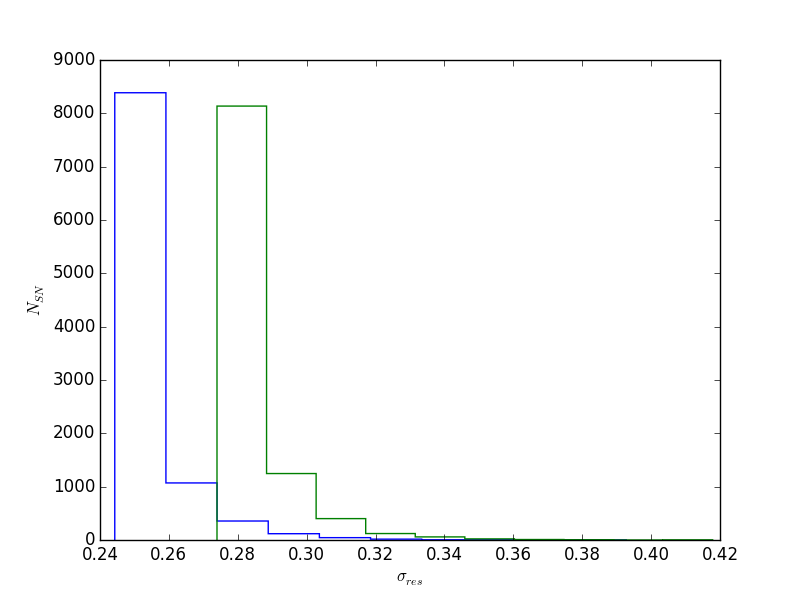
\includegraphics[width=0.6\textwidth]{../sigres.png}
\caption{Histogram of the samples for $\sigma_{res}$ using $t_2$ (blue) and $x_1$ (green)}
\label{fig:stan}
\end{figure}

The median for $t_2$ is 0.24 whereas for $x_1$ is 0.27 mag. Without correction the scatter is 0.31.
As a diagnostic, the pearson coefficient (r) for $t_2$ is 0.64, whereas for $x_1$ it is 0.51.
\end{document}